\section{Results}\label{results}

\begin{figure}[H]
  \centering
  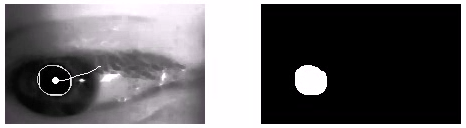
\includegraphics[width=0.9\textwidth]{fin_dark.png}
  \caption{Tracking of the pupil.}\label{fig:pupil1}
\end{figure}

\begin{figure}[H]
  \centering
  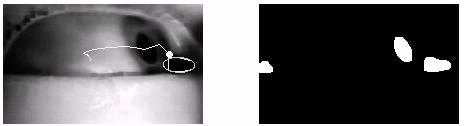
\includegraphics[width=0.9\textwidth]{fin_lost.png}
  \caption{Tracking of the pupil.}\label{fig:pupil1}
\end{figure}

\begin{figure}[H]
  \centering
  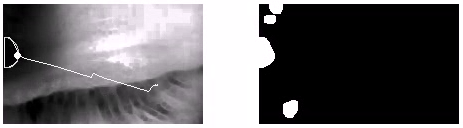
\includegraphics[width=0.9\textwidth]{fin_closed.png}
  \caption{Tracking of the pupil.}\label{fig:pupil1}
\end{figure}

\begin{figure}[H]
  \centering
  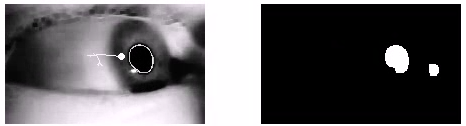
\includegraphics[width=0.9\textwidth]{fin_temporal.png}
  \caption{Tracking of the pupil.}\label{fig:pupil1}
\end{figure}

\begin{figure}[H]
  \centering
  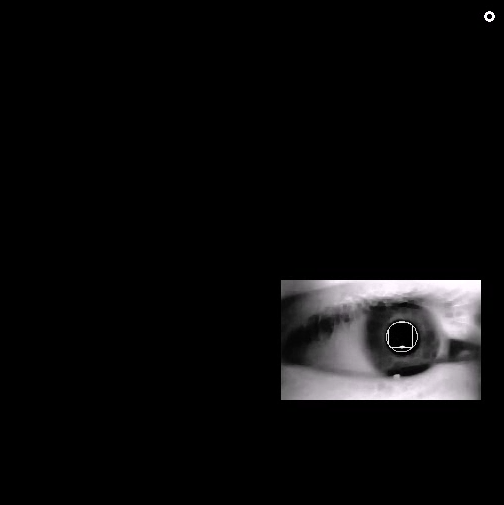
\includegraphics[width=0.9\textwidth]{fin_calibration.png}
  \caption{Tracking of the pupil.}\label{fig:pupil1}
\end{figure}

\begin{figure}[H]
  \centering
  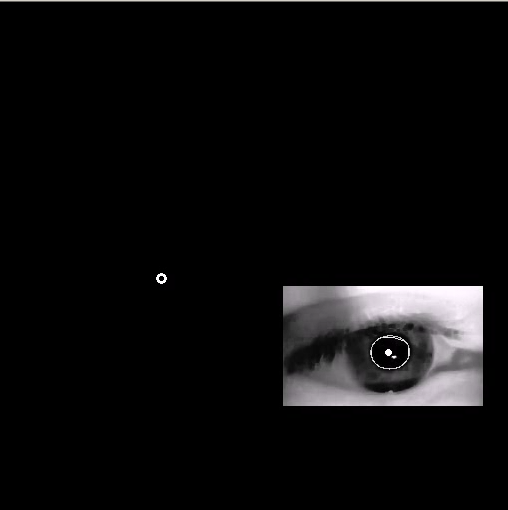
\includegraphics[width=0.9\textwidth]{fin_mapping.png}
  \caption{Tracking of the pupil.}\label{fig:pupil1}
\end{figure}

\begin{figure}[H]
  \centering
  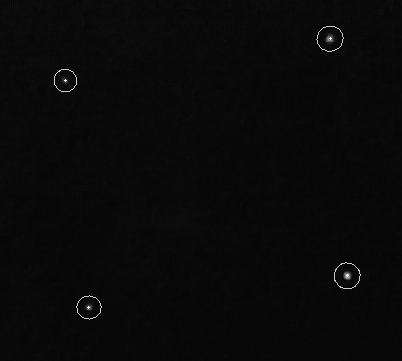
\includegraphics[width=0.9\textwidth]{fin_head.png}
  \caption{Tracking of the pupil.}\label{fig:pupil1}
\end{figure}

To get an idea of the whole process, please see the attached video. This video first shows how the eye tracking works in general. Some problems are shown as well, for instance the behaviour of the pupil tracking when the eye is closed or when the eye movement is too big and the tracking can not distinguish between the pupil and shadows. Keep in mind that movements this big do not occur in normal usage, as the movement of the eye is rather limited when looking at a computer screen.

The next part shows the calibration process, where the user has to look at several points on the screen.

After his process, all the necessary information is gathered to perform the mapping, which is shown subsequently. The user looks at several points on the screen and the position of the pupil is mapped onto the screen. 

The result shown in this video lacks the head tracking, as we weren't able to implement this properly due to several tough problems. These problems are discussed in the next section.


